\documentclass[english,xcolor=pst,11pt]{beamer}

%\usetheme{Rochester}
%\usetheme{Berkeley}
\usetheme{Berlin}
\usepackage{beamerthemesplit}


\usepackage[utf8]{inputenc}
\usepackage{amsmath, amssymb, bbm}
\usepackage{url}
\usepackage{hyperref}
\usepackage{physics, slashed}
\usepackage{graphicx}
\usepackage{hyperref}
\usepackage{placeins}
\usepackage{calc}
\usepackage{float}
\usepackage{xcolor}
%\usepackage{accents}
\usepackage{stackrel}
\usepackage{mathtools}
\usepackage{graphicx}
\usepackage{adjustbox}

\usepackage{tikz}
\usetikzlibrary{patterns,math,calc}
\usetikzlibrary{decorations.pathreplacing}
\usetikzlibrary{positioning}
\usetikzlibrary{decorations.pathmorphing}
\usetikzlibrary{decorations.markings}
\usetikzlibrary{arrows}
\renewcommand\epsilon\varepsilon % its probably not consistent in the tex code
\renewcommand\nabla\partial % its probably not consistent in the tex code


\addtobeamertemplate{navigation symbols}{}{%
    \usebeamerfont{footline}%
    \usebeamercolor[fg]{footline}%
    \hspace{1em}%
    \insertframenumber/\inserttotalframenumber
}

\title[CI/CD for the Grid Library]{Continuous Performance Monitoring of the Grid Library on a Supercomputer}
\author{\textbf{Simon Bürger}, Antonin Portelli}
\date{July 30th, Lattice 2024, Liverpool}

% \pdfinfo{
%   /Title    (Scattering in Lattice Systems)
%   /Author   (Simon Bürger)
% }

\newlength\leftsidebar
\newlength\rightsidebar
\makeatletter
\setlength\leftsidebar{\beamer@leftsidebar}
\setlength\rightsidebar{\beamer@rightsidebar}
\makeatother

\begin{document}

%\maketitle

\begin{frame}
 \titlepage

 \begin{tikzpicture}[remember picture, overlay]
    % Position the logos using node coordinates
    \node[anchor=south west, yshift=1cm, xshift=1cm] at (current page.south west) {
\includegraphics[width=2.4cm]{logos/stfc.png}};
    \node[anchor=south west, yshift=1cm, xshift=3.8cm] at (current page.south west) {
\includegraphics[width=1.8cm]{logos/dirac.png}};
    \node[anchor=south east, yshift=1cm, xshift=-3.8cm] at (current page.south east) {
\includegraphics[width=2.2cm]{logos/epcc.pdf}};
    \node[anchor=south east, yshift=1cm, xshift=-1cm] at (current page.south east) {
\includegraphics[width=2.4cm]{logos/edinburgh.pdf}};
  \end{tikzpicture}
\end{frame}

% \begin{frame}
%  \begin{block}{Overview}
%   \begin{enumerate}
%    \item Goals
%    \item Implementation using TeamCity
%    \item Performance monitoring
%   \end{enumerate}
%  \end{block}
%
% \end{frame}



\section{Motivation and Goals}

\begin{frame}
 \textbf{Our code base}
 \begin{itemize}
  \item \emph{Grid}: data parallel C++ container classes mapping efficiently to SIMD architectures including GPUs \url{https://github.com/paboyle/Grid}
  \item \emph{Hadrons}: Grid-based workflow management system for lattice field theory simulations \url{https://github.com/aportelli/Hadrons}
 \end{itemize}

 \begin{figure}[H]
	\centering
  %\input{plots/schemes/schemes_quenched}
  \adjustbox{trim={.00\width} {.0\height} {0.01\width} {.0\height},clip}%
    {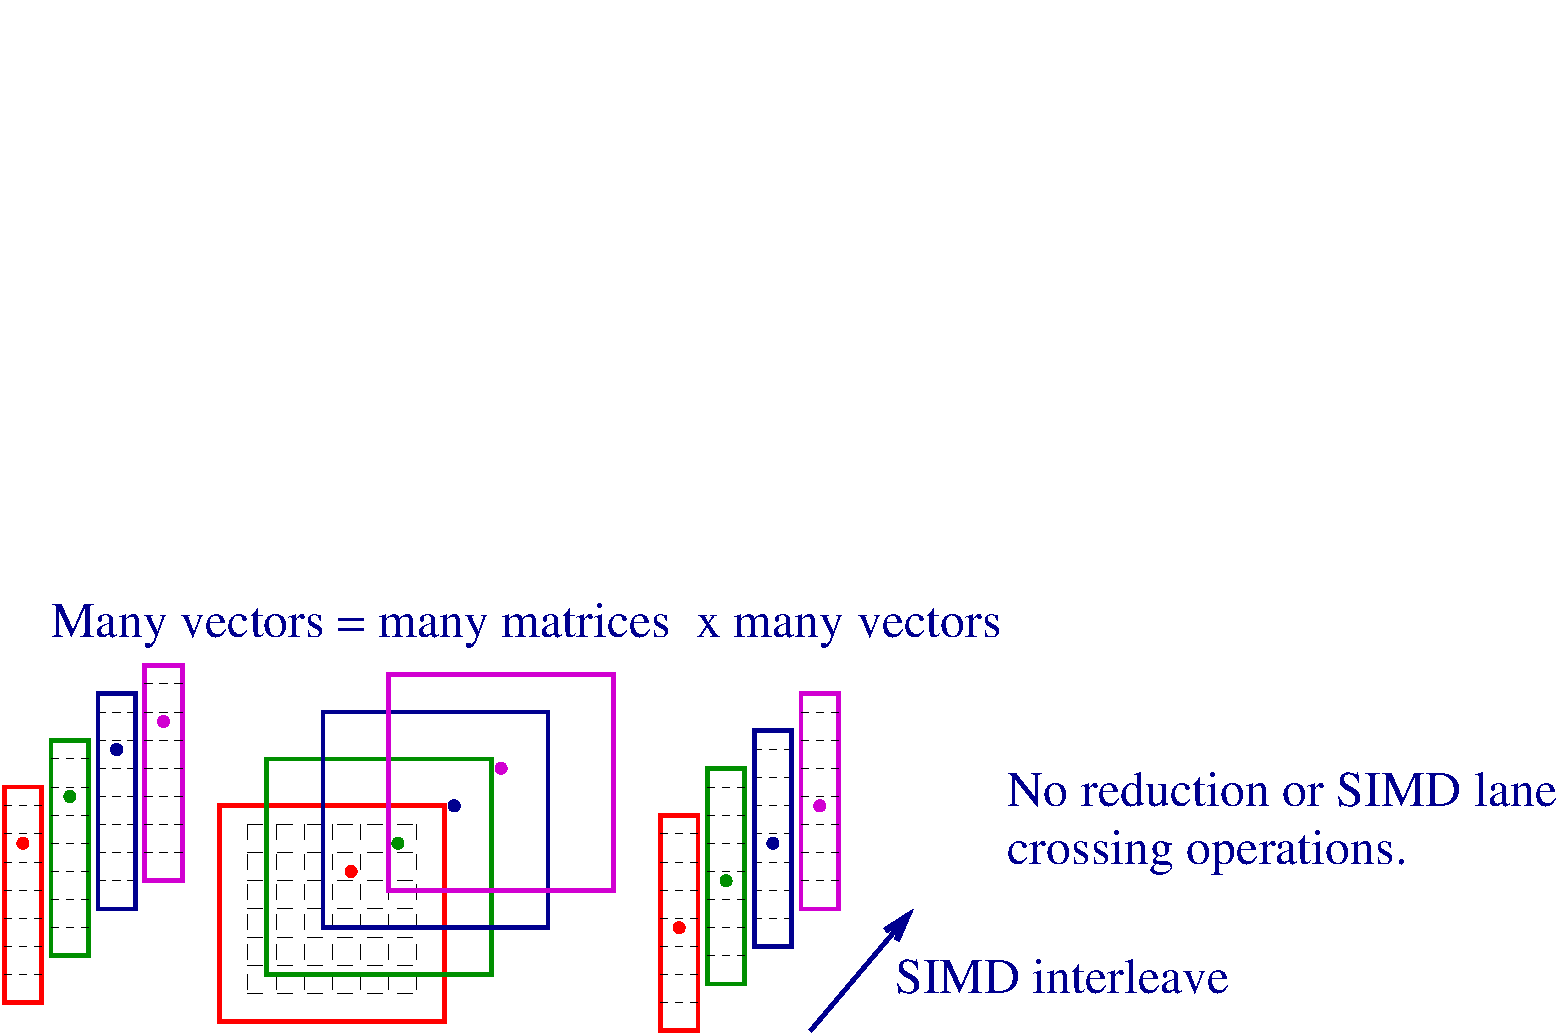
\includegraphics[width=3in]{diagrams/grid.pdf}}
    \caption{Grid architechture, from \url{[hep-lat/1512.03487]}}
\end{figure}
\end{frame}


\begin{frame}
 \textbf{Tursa Computing cluster}
 \begin{itemize}
  \item part of the national \emph{STFC DiRAC HPC facility}
  \item 178 compute nodes, each equipped with
  \begin{itemize}
    \item two \emph{AMD EPYC} processors
    \item four \emph{NVIDIA Ampere A100} accelerators
  \end{itemize}
  \item interconnect
  \begin{itemize}
   \item NVLink on each node, running at 600 GB/s
   \item Four HDR-200 infiniband interfaces per node
  \end{itemize}

  \item jobs are run via Slurm scheduler from dedicated login nodes
  \item find out more at \url{https://dirac.ac.uk}

 \end{itemize}

 \begin{tikzpicture}[remember picture, overlay]
    % Position the logos using node coordinates
    \node[anchor=south west, yshift=1cm, xshift=3cm] at (current page.south west) {
\includegraphics[width=2.4cm]{logos/stfc.png}};
    \node[anchor=south west, yshift=1cm, xshift=5.8cm] at (current page.south west) {
\includegraphics[width=1.8cm]{logos/dirac.png}};
  \end{tikzpicture}
\end{frame}

\begin{frame}

\textbf{Goals}
\begin{itemize}
 \item \textbf{Continuous integration}: Notice breaking changes as soon as possible, avoid infamous ``works on my machine''
 \item \textbf{Automatic deployment}: Improve reproducibility and simplify user experience
 \item \textbf{Performance monitoring}: Detect performance degredations caused by any part of the system
\end{itemize}

\end{frame}

\begin{frame}

\section{Jetbrains TeamCity}
\begin{minipage}{0.45\textwidth}

\textbf{Jetbrains TeamCity Architecture}
        \centering
        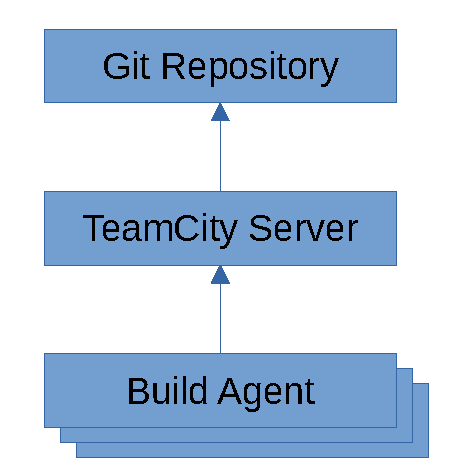
\includegraphics[width=0.9\textwidth]{diagrams/teamcity.pdf} % first figure itself
    \end{minipage}\hfill
    \begin{minipage}{0.45\textwidth}
        \centering
        
\includegraphics[width=0.9\textwidth]{logos/jetbrains.pdf}
        
\includegraphics[width=0.4\textwidth]{logos/teamcity.pdf}
        \end{minipage}

% \begin{figure}[H]
% 	\centering
%   %\input{plots/schemes/schemes_quenched}
%   %\adjustbox{trim={.01\width} {.35\height} {0.01\width} {.35\height},clip}%
%     {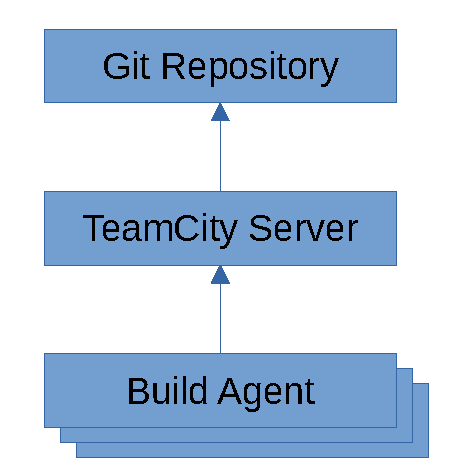
\includegraphics[width=1.8in]{diagrams/teamcity.pdf}}
% \end{figure}
\vfill
\begin{itemize}
 \item Scalable to arbitrary number of build servers
 \item Communication via https
\end{itemize}




\end{frame}

\begin{frame}
\textbf{Dedicated CICD hardware}
 \begin{figure}[H]
	\centering
  %\input{plots/schemes/schemes_quenched}
  %\adjustbox{trim={.01\width} {.35\height} {0.01\width} {.35\height},clip}%
    {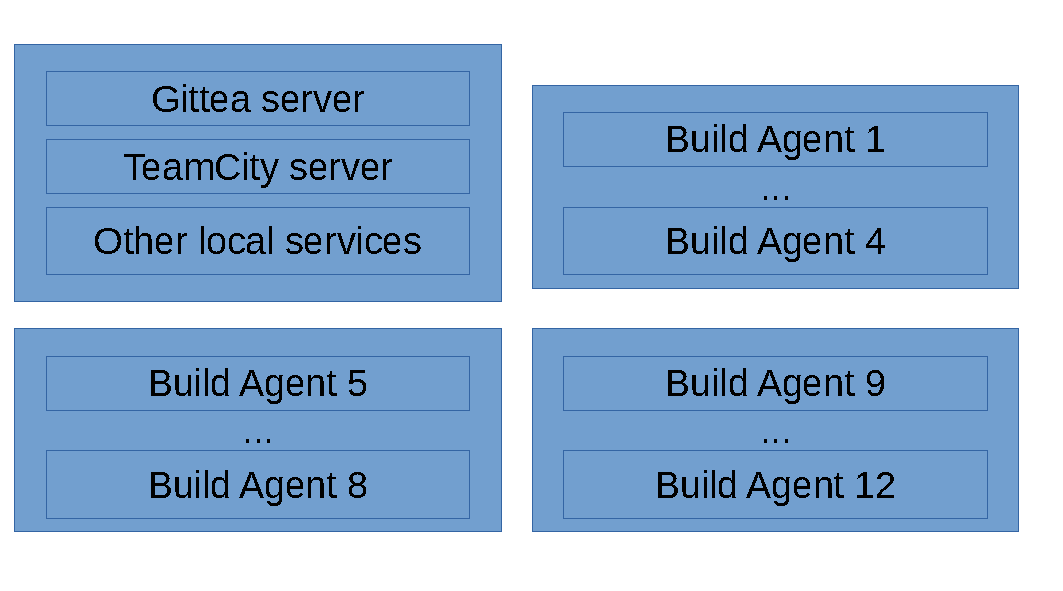
\includegraphics[width=3.2in]{diagrams/hardware.pdf}}
\end{figure}

\begin{itemize}
 \item Four AMD EPYC servers, same environment  as login nodes
 \item Head server: docker containers, externally visible
 \item Agents: run on bare metal, not externally visible
\end{itemize}

\end{frame}

\begin{frame}
 \textbf{Triggers for the CI system}
\begin{itemize}
 \item Each commit, including pending pull requests \\$\longrightarrow$ build Grid and Hadrons and run unittests
 \item Once per day: \\$\longrightarrow$ deploy new production binaries if there were any changes \\
 $\longrightarrow$ run benchmarks, using latest production binaries
 \item Benchmarking run regardless of code changes, thus monitoring the runtime environment as well.
\end{itemize}

\end{frame}




\section{HPC cluster integration}
\begin{frame}
 \textbf{Integration into the HPC cluster \emph{Tursa}}
 \begin{itemize}
  \item Problem: Build servers do not have GPUs
  \item Solution: GPU-based unittests and benchmarking jobs are submitted via SLURM to the computing cluster
  \item Finished jobs report back to TeamCity via a REST API
  \item Build agents are not waiting for SLURM queue
 \end{itemize}

\end{frame}

\section{Showcase}
\begin{frame}
 \textbf{What does it look like?}
 On a GitHub pull request:
  \begin{figure}[H]
	\centering
  %\input{plots/schemes/schemes_quenched}
  %\adjustbox{trim={.01\width} {.35\height} {0.01\width} {.35\height},clip}%
    {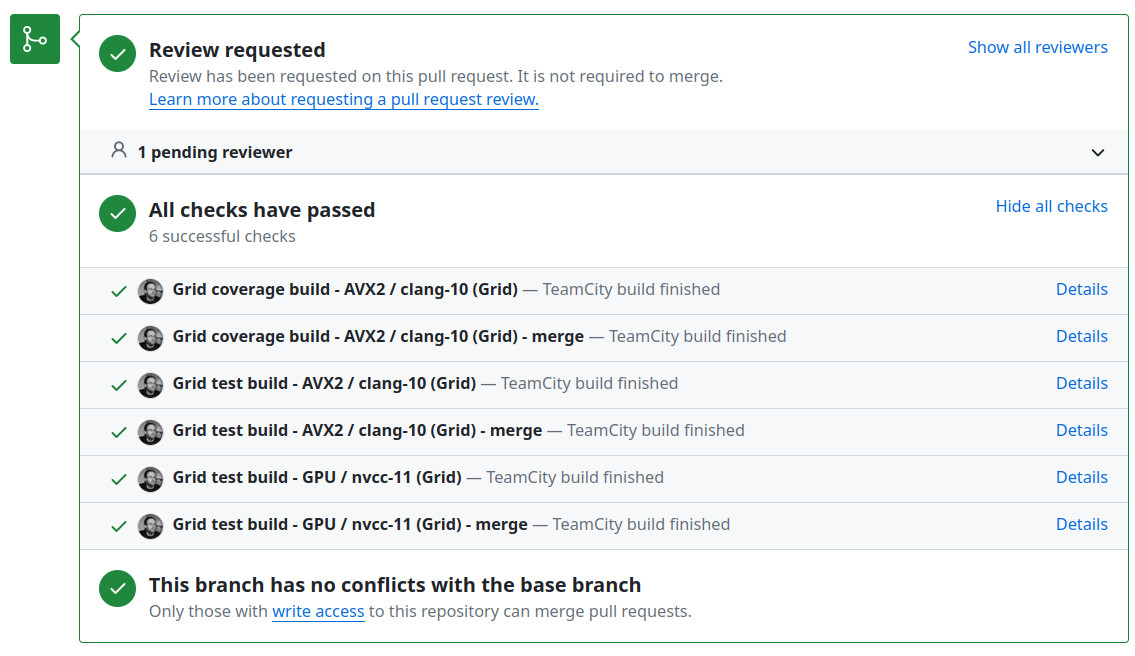
\includegraphics[width=4.3in]{diagrams/pr.jpg}}
\end{figure}
\end{frame}


{ % all template changes are local to this group.
    \setbeamertemplate{navigation symbols}{}
    \begin{frame}<article:0>[plain]
        \begin{tikzpicture}[remember picture,overlay]
            \node[at=(current page.center)] {
                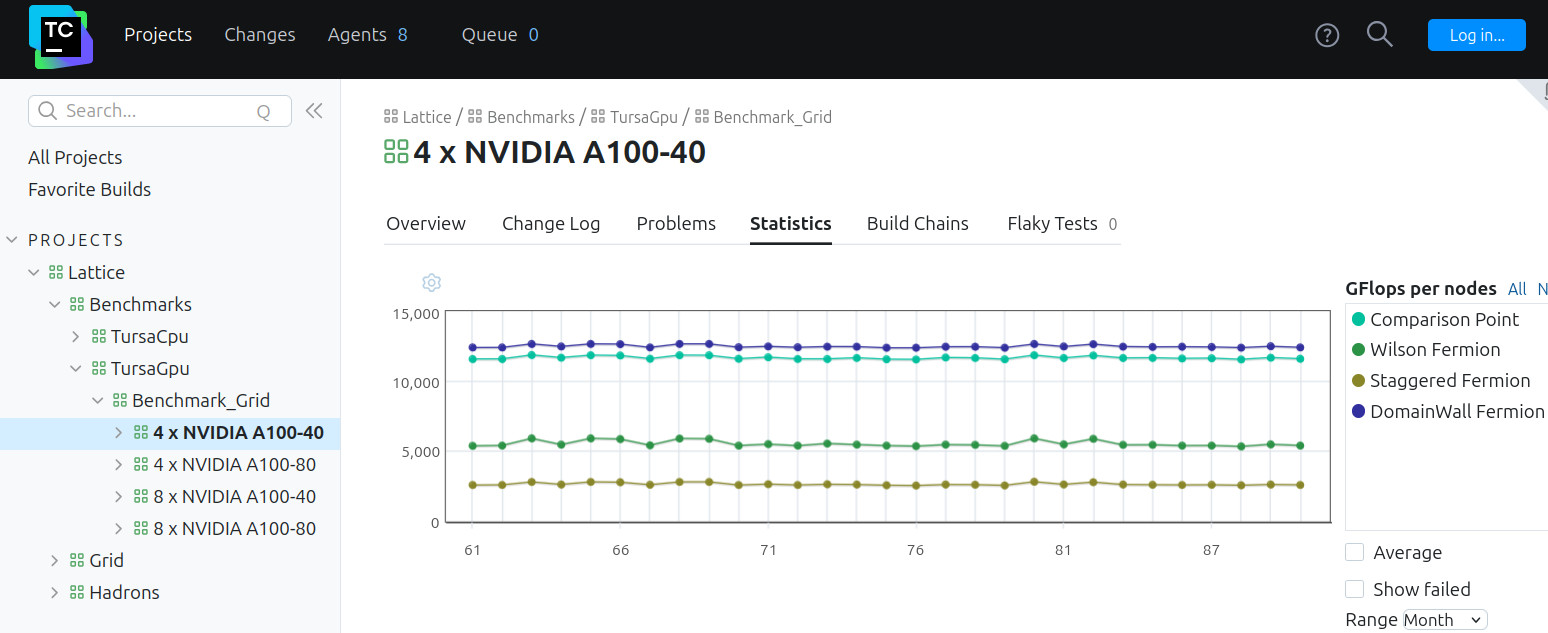
\includegraphics[keepaspectratio,
                                 width=\paperwidth,
                                 height=\paperheight]{diagrams/benchmarks.jpg}
            };
        \end{tikzpicture}
     \end{frame}
}

\section{Discussion}
\begin{frame}
 \textbf{Stability}
 \begin{itemize}
  \item All build artifacts are backed up to a cloud storage provider
  \item Configuration of TeamCity itself is tracked in a git repository
  \end{itemize}
  \textbf{Hardening}
  \begin{itemize}
  \item Build servers are not publicly visible, communication to main server is ``one-way''
  \item Build agents run as dedicated  user with limited permissions on the cluster, e.g., no access to research data
 \end{itemize}
 \textbf{Future outlook}

 \begin{itemize}
  \item Solution is scalable to multiple HPC clusters
 \end{itemize}
 \vfill
\emph{This CI/CD solution was funded by the STFC DiRAC Facility}
\end{frame}


\begin{frame}
\centering
 \Large{\textbf{Questions?}} \\ \vfill
 \small{for a live demo, come talk to me later, or visit \url{https://ci.dev.dirac.ed.ac.uk} \\(choose ``Log in as guest'')}

 \begin{tikzpicture}[remember picture, overlay]
    % Position the logos using node coordinates
    \node[anchor=south west, yshift=1cm, xshift=1cm] at (current page.south west) {
\includegraphics[width=2.4cm]{logos/stfc.png}};
    \node[anchor=south west, yshift=1cm, xshift=3.8cm] at (current page.south west) {
\includegraphics[width=1.8cm]{logos/dirac.png}};
    \node[anchor=south east, yshift=1cm, xshift=-3.8cm] at (current page.south east) {
\includegraphics[width=2.2cm]{logos/epcc.pdf}};
    \node[anchor=south east, yshift=1cm, xshift=-1cm] at (current page.south east) {
\includegraphics[width=2.4cm]{logos/edinburgh.pdf}};
  \end{tikzpicture}

\end{frame}




\end{document}
